\documentclass[a6paper,10pt]{article}
%\usepackage[T1]{fontenc}
\usepackage[british]{babel}
\usepackage[utf8]{inputenc}
\usepackage{float, graphicx,amsmath,amsfonts,cite,enumerate,tabularx}
\usepackage[final]{pdfpages}
\usepackage{wrapfig}
\usepackage[margin=0.3in]{geometry}
\usepackage{../sidspaltHack}
\newcommand{\mel}[1]{\small\textbf{\textit{mel. #1 \\}}}


\setlength{\oddsidemargin}{-0.37in}
\setlength{\textwidth}{215pt}

\pagestyle{empty}

\begin{document}
\nysida{6}{1}
\noindent
\huge{Z$\zeta$ Visor till punsch}
\begin{center}
\Large $\zeta1$. Punschen kommer \\ 
\mel{Glada änkan}
\end{center}
\small Punschen kommer, punschen kommer,\\
ljuv och sval.\\
Glasen imma, röster stimma,\\
i vår sal.\\
Skål för glada minnen,\\
skål för varje vår!\\
Inga sorger finnas mer\\
när punsch vi får.
\vspace{10pt}\\
\textit{Sjungs medan punschen serveras, under det att en gungar vänster-höger, framåt-bakåt och uppåt-nedåt.
\vspace{5pt}\\
Den som fått sin punsch slutar sjunga.}

\nysida{6}{2}
\setlength{\oddsidemargin}{-0.47in}
\noindent
\begin{center}
\Large $\zeta2$. Punschhkanon \\ 
\mel{Gökvisa}
\end{center}
\textit{Herrar:}
\vspace{4pt}\\
$\|$: Punsch punsch punsch punsch\\
punsch punsch, alla sorters :$\|$
\vspace{5pt}\\
\textit{Damer:}
\vspace{4pt}\\
När snapsen vandrat hädan\\
och maten lagts därpå\\
och kaffet står på bordet\\
vad väntar vi då på?
\vspace{5pt}\\
$\|$: Jo, punsch, och punsch\\
och ännu mera punsch. :$\|$
\vspace{5pt}\\
Ja den föll oss i smaken \\
nu ropar vi gutår\\
och koppen står där naken\\
och väntar på påtår.
\vspace{5pt}\\
Jo punsch...
\vspace{10pt}\\
\textit{En sann gentleman ger damerna förstärkning om det behövs.}
\begin{figure}[!h]
\centering
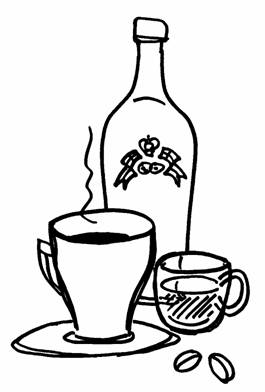
\includegraphics[width=0.35\textwidth]{kaffe.jpg}
\end{figure}

\nysida{6}{3}
\setlength{\oddsidemargin}{-0.37in}
\noindent
\begin{center}
\Large $\zeta3$. Punschschottis \\ 
\mel{Schottis på Valhall}
\end{center}
Uppå bordet står nu en liten tår\\
den har lyster precis som en kristall.\\
Den är lockande, den är pockande,\\
och fast den är isande kall.\\
Den oss värme ger när den slunkit ner\\
i en dammig och torr liten hals.\\
Det är punschen som går.\\
Det är punschen som fårä\\
hela livet att bli till en vals.
\vspace{40pt}
\begin{center}
\Large $\zeta4$. Punschens lov \\ 
\mel{Rövarvisan}
\end{center}
$\|$: Punsch, punsch, punsch, punsch :$\|$
\vspace{5pt}\\
Punschen är och punschen var\\
och punschen skall förbliva\\
en lidelse vi alla har\\
som ingen kan fördriva.
\vspace{5pt}\\
Ja, punschen tinar upp så väl\\
och svalkar både kropp och själ.\\
Det botar begären\\
och lindrar besvären.\\
Ja punschen den gör både gott och väl.
\begin{flushright}
\textit{Kårspexet Sven Hedin 1987}
\end{flushright}

\nysida{6}{5}
\setlength{\oddsidemargin}{-0.47in}
\noindent
\begin{center}
\Large $\zeta5$. Jag gillar punschen \\ 
\end{center}
Länge har jag tänkt\\
att punschen övergiva,\\
men det blir aldrig av\\
så länge jag får leva.\\
För när jag en gång dör\\
så står det på min grav:\\
"Här vilar en som\\
Svenska punschen gillat har."
\vspace{5pt}\\
Jag gillar, jag gillar punschen,\\
jag gillar den som punschen skapat har.\\
Jag gillar, jag gillar punschen,\\
jag gillar punschen och dess far.
\begin{flushright}
\textit{Ur Skogshögskolans sångbok 1906}
\end{flushright}
\vfill
\begin{center}
\Large $\zeta6$. Imperial punsch \\ 
\mel{Imperial March (Star Wars)}
\end{center}
Punsch, punsch, punsch, mera punsch, mera punsch!\\
Punsch, punsch, punsch, mera punsch, mera punsch!
\vspace{5pt}\\
Punsch, punsch, punsch, mera punsch,\\
punsch punsch,\\
mera punsch, punsch, punsch, mera punsh,\\
mera punsch!
\begin{flushright}
\textit{DKM 2000}
\end{flushright}

\nysida{6}{7}
\setlength{\oddsidemargin}{-0.37in}
\noindent
\begin{center}
\Large $\zeta7$. Djungelpunsch \\ 
\mel{Var nöjd med.../Djungelboken}
\end{center}
Jag gillar alla tiders punsch.\\
Punsch till frukost, punsch till lunch.\\
En punsch till förrätt, varmrätt och dessert.\\
Jag gillar punsch för vet du vad;\\
rent kaffe gör ju ingen glad.\\
Så punsch för fulla muggar vill jag ha!
\vspace{5pt}\\
Med konjak du lockar\\
den bästa Renault.\\
Förlåt om jag chockar\\
och tar punsch ändå.\\
Och bjuder du på nån förnäm likör\\
så får du ursäkta det kanske stör\\
men jag väljer hellre Grönstedts blå,\\
en cederlunds eller Flaggpunsch åh...\\
kanske har du ren platin?\\
Jag gillar punsch,\\
så ge mig punsch\\
och jag är din,\\
för evigt din.\\

\nysida{6}{8}
\setlength{\oddsidemargin}{-0.47in}
\noindent

\begin{center}
\Large $\zeta8$. Vi vill ha punsch \\ 
\mel{Theme from the Addams family}
\end{center}
Vi vill ha punsch. \textit{(knäpp, knäpp)}\\
Vi vill ha punsch. \textit{(knäpp, knäpp)}\\
Vi vill ha punsch, vi vill ha punsch.\\
Vi vill ha punsch. \textit{(knäpp, knäpp)}
\vspace{5pt}\\
När en vill festen liva,\\
upp är det bra att kliva\\
omkring på bordets skiva\\
och klafsa runt i punsch.
\vspace{5pt}\\
Klafsa i punsch. \textit{(slurp, slurp)}\\
Klafsa i punsch. \textit{(slurp, slurp)}\\
Klafsa i punsch, klafsa i punsch.\\
Klafsa i punsch. \textit{(slurp, slurp)}

\begin{center}
\Large $\zeta9$. Punsch, punsch \\ 
\mel{Ritsch, ratsch}
\end{center}
Punsch, punsch filibombombom,\\
filibombombom, filibombombom.\\
Punsch, punsch filibombombom,\\
filibombombom, filibom!
\vspace{5pt}\\
Vi har ju både \\
Cederlunds och Carlshamns flagg\\
och Grönstedts blå\\
och lilla Caloric.\\
Det blir för trist med sodavatten,\\
sodavatten, sodavatten.\\
Blir för trist med sodavatten,\\
ge mig lite punsch!

\nysida{6}{10}
\setlength{\oddsidemargin}{-0.37in}
\noindent

\begin{center}
\Large $\zeta10$. Studiemedelsrondo \\ 
\mel{Lossa sand}
\end{center}
Vi dricker punsch till lunch\\
när vi har fått avin.\\
Vi lunchar hela dagen\\
tills kassan gått i sin.
\vspace{10pt}\\
\textit{Upprepas, allt snabbare}
\vspace{40pt}
\begin{center}
\Large $\zeta11$. FESTU:s punschvisa \\ 
\mel{Tomtarnas julnatt}
\end{center}
Punschen, punschen,\\
rinner genom strupen, \\
ner i djupen.\\
Blandas, konfronteras\\
där med supen,\\
där med supen.\\
Gula droppar\\
stärker våra kroppar!\\
Punsch, punsch, punsch!

\nysida{6}{12}
\setlength{\oddsidemargin}{-0.47in}
\noindent

\begin{center}
\Large $\zeta12$. Visa en torsdagskväll \\ 
\mel{Visa vid midsommartid}
\end{center}
Du häller ur flaskan en gyllene tår\\
av punsch ifrån Cederlunds.\\
Du lyfter sen bägarn och väl du förstår\\
att föra den till din mun.\\
Ikväll ska du dricka ditt livselixir\\
och känna den ljuva punschen\\
som ett vårbjörkeskir.\\
I natt ska du bäras av Osquarulda på bår\\
och kallas för fyllefår.
\vspace{40pt}
\begin{center}
\Large $\zeta13$. Sveriges Arraktionalhymn \\ 
\mel{Du gamla, Du fria}
\end{center}
Du ädla, du friska, du livselixir,\\
med dig vill jag mina läppar blöta.\\
Den svenskaste drycken på jorden, den förblir\\
den gyllene, den underbara söta,\\
den gyllene, den underbara söta.
\vspace{5pt}\\
Som iskallt till kaffet du ställs på vårt bord\\
och även som varm till torsdagslunchen.\\
Jag halsar dig lenaste drycken uppå jord.\\
Ja, jag vill leva, jag vill dö av punschen.\\
Ja, jag vill leva, jag vill dö av punschen.
\begin{flushright}
\textit{Ekonomspexet Erik XIV, 1992}
\end{flushright}

\nysida{6}{1/$\varepsilon$}
\setlength{\oddsidemargin}{-0.37in}
\noindent
\begin{center}
\Large $\zeta1/\varepsilon$. Punschfinalen \\ 
\mel{Rysslands nationalsång}
\end{center}
Ikväll har Napoleon gjort England den äran\\
att komma på middag till dess ambassad.\\
Men nu har ni sett till allas förfäran\\
att blott tomma flaskor står på parad.
\vspace{5pt}\\
Så går vi ner, ner till stadens hamnkvarter\\
och vid kajen Victory vi ser.\\
Vi går ombord och där väntar ett Nachspiel på oss.\\
Vi går till bords både fiende och vän\\
och våra gräl dom sparar vi till sen.\\
Vi tar en matbit, en sup, nej flera förtås.
\vspace{5pt}\\
Idag har lord Nelson krökat i Neapel.\\
Han raglar omkring med armen i en slips.\\
Men snart står han uppsträckt i London på en stapel,\\
vi undrar om någon i groggen har lagt gips.
\vspace{5pt}\\
Så går vi ner...
\begin{flushright}
\textit{Bergsspexet Lord Nelson 1975}
\end{flushright}

\nysida{6}{$\infty$}
\setlength{\oddsidemargin}{-0.47in}
\noindent
\begin{center}
\Large $\zeta\infty$. Sista punschvisan \\ 
\mel{Auld lang syne}
\end{center}
När punschen småningom ta't slut\\
och vår flaska blivit tom.\\
Då vänder vi den upp och ner\\
till dess inget rinner ut.
\vspace{5pt}\\
$\|$: Så slicka vi, så slicka vi,\\
båd' utanpå och i.\\
Och finns det ändå något kvar\\
får det va' till sämre dar. :$\|$
\vspace{10pt}\\
\textit{Andra versen brukar sjungas två gånger på fina sittningar. På mer uppsluppna fester sjungs andra versen\\
$\cdot$ sittande\\
$\cdot$ stående\\
$\cdot$ med en fot på stolen\\
$\cdot$ med båda fötter på stolen\\
$\cdot$ med en fot på bordet\\
$\cdot$ och till sist under bordet}
\end{document}